% Name: Parabola, focus, and directrix
% Description: The parabola x² = 4py is the set of points P as far from the focus F as from the directrix y = −p.
% Tags: conic section, parabola, focus, directrix

\usetikzlibrary{arrows.meta}

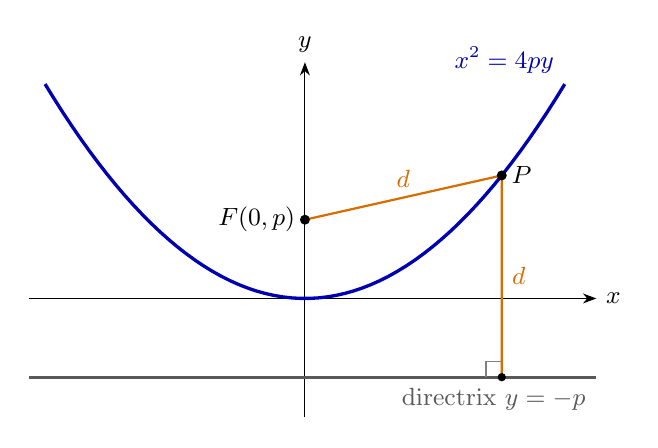
\begin{tikzpicture}[>={Stealth}, every node/.style={font=\small}]
  % p = 1: focus (0, 1), directrix y = -1; P = (2.5, 2.5^2/4) is 2.5625 from both
  \coordinate (F) at (0,1);
  \coordinate (P) at (2.5,1.5625);
  \coordinate (D) at (2.5,-1);
  \draw[->] (-3.5,0) -- (3.7,0) node[right] {$x$};
  \draw[->] (0,-1.5) -- (0,3) node[above] {$y$};
  \draw[very thick, blue!70!black, domain=-3.3:3.3, samples=60] plot (\x,{\x*\x/4}) node[above left] {$x^2 = 4py$};
  \draw[very thick, gray!70!black] (-3.5,-1) -- (3.7,-1) node[below left] {directrix $y = -p$};
  \draw[thick, orange!85!black] (F) -- node[above] {$d$} (P) -- node[right] {$d$} (D);
  \draw[gray] (D) ++(-0.2,0) |- ++(0.2,0.2);
  \fill (F) circle (1.8pt) node[left] {$F(0, p)$};
  \fill (P) circle (1.8pt) node[right] {$P$};
  \fill (D) circle (1.5pt);
\end{tikzpicture}
